% A LaTeX (non-official) template for ISAE projects reports
% Copyright (C) 2014 Damien Roque
% Version: 0.2
% Author: Damien Roque <damien.roque_AT_isae.fr>

\documentclass[a4paper,12pt]{book}
\usepackage[utf8]{inputenc}
\usepackage[T1]{fontenc}
\usepackage[frenchb]{babel} % If you write in French
%\usepackage[english]{babel} % If you write in English
\usepackage{a4wide}
\usepackage{graphicx}
\graphicspath{{images/}}
\usepackage{subfig}
\usepackage{tikz}
\usetikzlibrary{shapes,arrows}
\usepackage{pgfplots}
\pgfplotsset{compat=newest}
\pgfplotsset{plot coordinates/math parser=false}
\newlength\figureheight
\newlength\figurewidth
\pgfkeys{/pgf/number format/.cd,
set decimal separator={,\!},
1000 sep={\,},
}

\usepackage{listings}
\usepackage{xcolor}
\lstset { %
    language=C++,
    basicstyle=\ttfamily,
    keywordstyle=\color{blue}\ttfamily,
    stringstyle=\color{red}\ttfamily,
    commentstyle=\color{green}\ttfamily,
    numbers=left,
    morecomment=[l][\color{magenta}]{\#}
}

\usepackage{ifthen}
\usepackage{ifpdf}
\ifpdf
\usepackage[pdftex]{hyperref}
\else
\usepackage{hyperref}
\fi
\usepackage{color}
\hypersetup{%
colorlinks=true,
linkcolor=black,
citecolor=black,
urlcolor=black}

\renewcommand{\baselinestretch}{1.05}
\usepackage{fancyhdr}
\pagestyle{fancy}
\fancyfoot{}
\fancyhead[LE,RO]{\bfseries\thepage}
\fancyhead[RE]{\bfseries\nouppercase{\leftmark}}
\fancyhead[LO]{\bfseries\nouppercase{\rightmark}}
\setlength{\headheight}{15pt}

\let\headruleORIG\headrule
\renewcommand{\headrule}{\color{black} \headruleORIG}
\renewcommand{\headrulewidth}{1.0pt}
\usepackage{colortbl}
\arrayrulecolor{black}

\fancypagestyle{plain}{
  \fancyhead{}
  \fancyfoot[C]{\thepage}
  \renewcommand{\headrulewidth}{0pt}
}

\makeatletter
\def\@textbottom{\vskip \z@ \@plus 1pt}
\let\@texttop\relax
\makeatother

\makeatletter
\def\cleardoublepage{\clearpage\if@twoside \ifodd\c@page\else%
  \hbox{}%
  \thispagestyle{empty}%
  \newpage%
  \if@twocolumn\hbox{}\newpage\fi\fi\fi}
\makeatother

\usepackage{amsthm}
\usepackage{amssymb,amsmath,bbm}
\usepackage{array}
\usepackage{bm}
\usepackage{multirow}
\usepackage[footnote]{acronym}

\newcommand*{\SET}[1]  {\ensuremath{\mathbf{#1}}}
\newcommand*{\VEC}[1]  {\ensuremath{\boldsymbol{#1}}}
\newcommand*{\FAM}[1]  {\ensuremath{\boldsymbol{#1}}}
\newcommand*{\MAT}[1]  {\ensuremath{\boldsymbol{#1}}}
\newcommand*{\OP}[1]  {\ensuremath{\mathrm{#1}}}
\newcommand*{\NORM}[1]  {\ensuremath{\left\|#1\right\|}}
\newcommand*{\DPR}[2]  {\ensuremath{\left \langle #1,#2 \right \rangle}}
\newcommand*{\calbf}[1]  {\ensuremath{\boldsymbol{\mathcal{#1}}}}
\newcommand*{\shift}[1]  {\ensuremath{\boldsymbol{#1}}}

\newcommand{\eqdef}{\stackrel{\mathrm{def}}{=}}
\newcommand{\argmax}{\operatornamewithlimits{argmax}}
\newcommand{\argmin}{\operatornamewithlimits{argmin}}
\newcommand{\ud}{\, \mathrm{d}}
\newcommand{\vect}{\text{Vect}}
\newcommand{\sinc}{\ensuremath{\mathrm{sinc}}}
\newcommand{\esp}{\ensuremath{\mathbb{E}}}
\newcommand{\hilbert}{\ensuremath{\mathcal{H}}}
\newcommand{\fourier}{\ensuremath{\mathcal{F}}}
\newcommand{\sgn}{\text{sgn}}
\newcommand{\intTT}{\int_{-T}^{T}}
\newcommand{\intT}{\int_{-\frac{T}{2}}^{\frac{T}{2}}}
\newcommand{\intinf}{\int_{-\infty}^{+\infty}}
\newcommand{\Sh}{\ensuremath{\boldsymbol{S}}}
\newcommand{\C}{\SET{C}}
\newcommand{\R}{\SET{R}}
\newcommand{\Z}{\SET{Z}}
\newcommand{\N}{\SET{N}}
\newcommand{\K}{\SET{K}}
\newcommand{\reel}{\mathcal{R}}
\newcommand{\imag}{\mathcal{I}}
\newcommand{\cmnr}{c_{m,n}^\reel}
\newcommand{\cmni}{c_{m,n}^\imag}
\newcommand{\cnr}{c_{n}^\reel}
\newcommand{\cni}{c_{n}^\imag}
\newcommand{\tproto}{g}
\newcommand{\rproto}{\check{g}}
\newcommand{\LR}{\mathcal{L}_2(\SET{R})}
\newcommand{\LZ}{\ell_2(\SET{Z})}
\newcommand{\LZI}[1]{\ell_2(\SET{#1})}
\newcommand{\LZZ}{\ell_2(\SET{Z}^2)}
\newcommand{\diag}{\operatorname{diag}}
\newcommand{\noise}{z}
\newcommand{\Noise}{Z}
\newcommand{\filtnoise}{\zeta}
\newcommand{\tp}{g}
\newcommand{\rp}{\check{g}}
\newcommand{\TP}{G}
\newcommand{\RP}{\check{G}}
\newcommand{\dmin}{d_{\mathrm{min}}}
\newcommand{\Dmin}{D_{\mathrm{min}}}
\newcommand{\Image}{\ensuremath{\text{Im}}}
\newcommand{\Span}{\ensuremath{\text{Span}}}

\newtheoremstyle{break}
  {11pt}{11pt}%
  {\itshape}{}%
  {\bfseries}{}%
  {\newline}{}%
\theoremstyle{break}

%\theoremstyle{definition}
\newtheorem{definition}{Définition}[chapter]

%\theoremstyle{definition}
\newtheorem{theoreme}{Théorème}[chapter]

%\theoremstyle{remark}
\newtheorem{remarque}{Remarque}[chapter]

%\theoremstyle{plain}
\newtheorem{propriete}{Propriété}[chapter]
\newtheorem{exemple}{Exemple}[chapter]

\parskip=5pt
%\sloppy

\begin{document}

%%%%%%%%%%%%%%%%%%
%%% First page %%%
%%%%%%%%%%%%%%%%%%

\begin{titlepage}
\begin{center}


\begin{figure}[h]
    \begin{minipage}[c]{.46\linewidth}
        \centering
        
\includegraphics[width=1\textwidth]{logo_ucp.jpg}
    \end{minipage}
    \hfill%
    \begin{minipage}[c]{.46\linewidth}
        \centering
        
\includegraphics[width=1\textwidth]{logo_echo.png}
    \end{minipage}
\end{figure}

{\large Dossier de projet associatif par l'association étudiante >ECHO}\\[0.5cm]

%{\large Type de projet}\\[0.5cm]

% Title
\rule{\linewidth}{0.5mm} \\[0.4cm]
{ \huge \bfseries Nom du projet \\[0.4cm] }
\rule{\linewidth}{0.5mm} \\[1.5cm]

% Author and supervisor
\noindent
\begin{minipage}{0.4\textwidth}
    \centering
    \includegraphics[width=1\textwidth]{logo_projet.jpg}
\end{minipage}%

\vfill

% Bottom of the page
{\large \today}

\end{center}
\end{titlepage}

%%%%%%%%%%%%%%%%%%%%%%%%%%%%%
%%% Non-significant pages %%%
%%%%%%%%%%%%%%%%%%%%%%%%%%%%%

\frontmatter

\clearpage
\tableofcontents

%\clearpage
%\listoffigures

%\clearpage
%\chapter*{Liste des sigles et acronymes}
%\begin{acronym}[CP-OFDMX] % Give the longest acronym here
%\acro{VR}{\emph{Virtual Reality}}
%\end{acronym}

%%%%%%%%%%%%%%%%%%%%%%%%%%%%%%%%%%%%%%%%%%%%
%%% Content of the report and references %%%
%%%%%%%%%%%%%%%%%%%%%%%%%%%%%%%%%%%%%%%%%%%%

\mainmatter
\pagestyle{fancy}

%\cleardoublepage

\chapter*{Introduction}
\addcontentsline{toc}{chapter}{Introduction}
\markboth{Introduction}{Introduction}
\label{chap:introduction}
%\minitoc



%%% Local Variables: 
%%% mode: latex
%%% TeX-master: "isae-report-template"
%%% End: 

\chapter{>ECHO}

% Corrigé

\label{chap:entreprise}
\begin{figure}[h]
    \centering
    
\includegraphics[width=0.65\textwidth]{images/logo_echo.png}
    \caption{Logo >ECHO}
\end{figure}
\section{Présentation}

    L'association >ECHO a été créer en 2009 par Jérôme FELLUS et d'autres étudiants en informatique afin de proposer une association qui pouvait les représenter et leur permettre de mieux s'intégrer et se rencontrer à l'Université de Cergy-Pontoise.
    
    Les manifestations qu'ECHO proposait à cette période étaient diverses et variées mais principalement liées à l'informatique et à la musique comme par exemple des "Installe Linux Party", dont le but était d'aider les nouveaux étudiants à installer le système d'exploitation Linux sur leurs machines, ou encore l'organisation de concert à la 33tour, salle de concert de l'Université de Cergy-Pontoise.
    
    En 2014, Johan CLOOTS, et les étudiants en 2\up{ème} année de licence d'informatique en cursus CMI ont repris l'association, qui était devenu inactive, dans le but d'animer le campus Saint-Martin. C'est à cette période que la première LAN Versity a été organisé. Ils ont réalisé de nombreuses coopératives mais aussi une semaine culturelle sur le thème de la musique avec une exposition de photos, la venue d'une artiste maquilleuse ou encore une jam session.
    
    En 2016, Alexandre FOURGS et Julien ABADJI, tous deux passionnées par la musique électronique et membre ou bénévole dans l'association >ECHO depuis 2 ans, ont repris l'association afin de faire perdurer les VersityLAN et de proposer des nouvelles manifestations sur le thème de la musique électronique à l'image de Cadence, un événement festif réalisé dans le restaurant universitaire de Saint-Martin où pour l'occasion une scène a été installée et des artistes du monde de la musique électronique se sont produits devant plus de 180 étudiants.
    
    D'une manière générale, l'association est très attaché à l'Université de Cergy-Pontoise et son animation, ses dirigeants ont depuis toujours proposé des événements au sein même de l'Université, quelle que soit la difficulté de l'organisation.
    
\newpage

\section{Objectifs}

    L'association >ECHO à deux "pôles" en son sein : le premier concerne l'informatique, le second la musique électronique.

    \subsection{Informatique}
    
        L'association >ECHO travaille en étroite collaboration avec les services du département informatique pour proposer aux étudiants des manifestations liées aux domaines de l'informatique et pour que ces derniers puissent se rencontrer et passer de bons moments ensemble, à l'image du barbecue du département informatique qui a lieu chaque année et où >ECHO a pu proposer diverses activités (exposition de memes, animations musicales, jeux vidéo, etc.).
        
        Le département informatique nous demande aussi son aide pour des événements comme les stages d'intégrations pour les nouveaux étudiants en informatique.
        
        L'association >ECHO est aussi là pour aider les étudiants en informatique en général.
        
        \subsubsection{VersityLAN}
        
            \begin{figure}[ht]
                \centering
                
\includegraphics[width=0.65\textwidth]{images/logo_versity.jpg}
                \caption{Logo Versity}
            \end{figure}
        
            L'association propose des événements liées à la culture du jeu vidéo, qui est très ancrée chez les informaticiens. 
            
            Durant l'année universitaire 2014-2015, >ECHO a réalisée ses deux premières LANs dans les locaux de l'Université qui ont rassemblées respectivement une trentaine et une cinquantaine d'étudiants de 18h à 00h sur des jeux comme League of Legends ou encore Counter Strike : Global Offensive.
            
            \begin{figure}[ht]
                \centering
                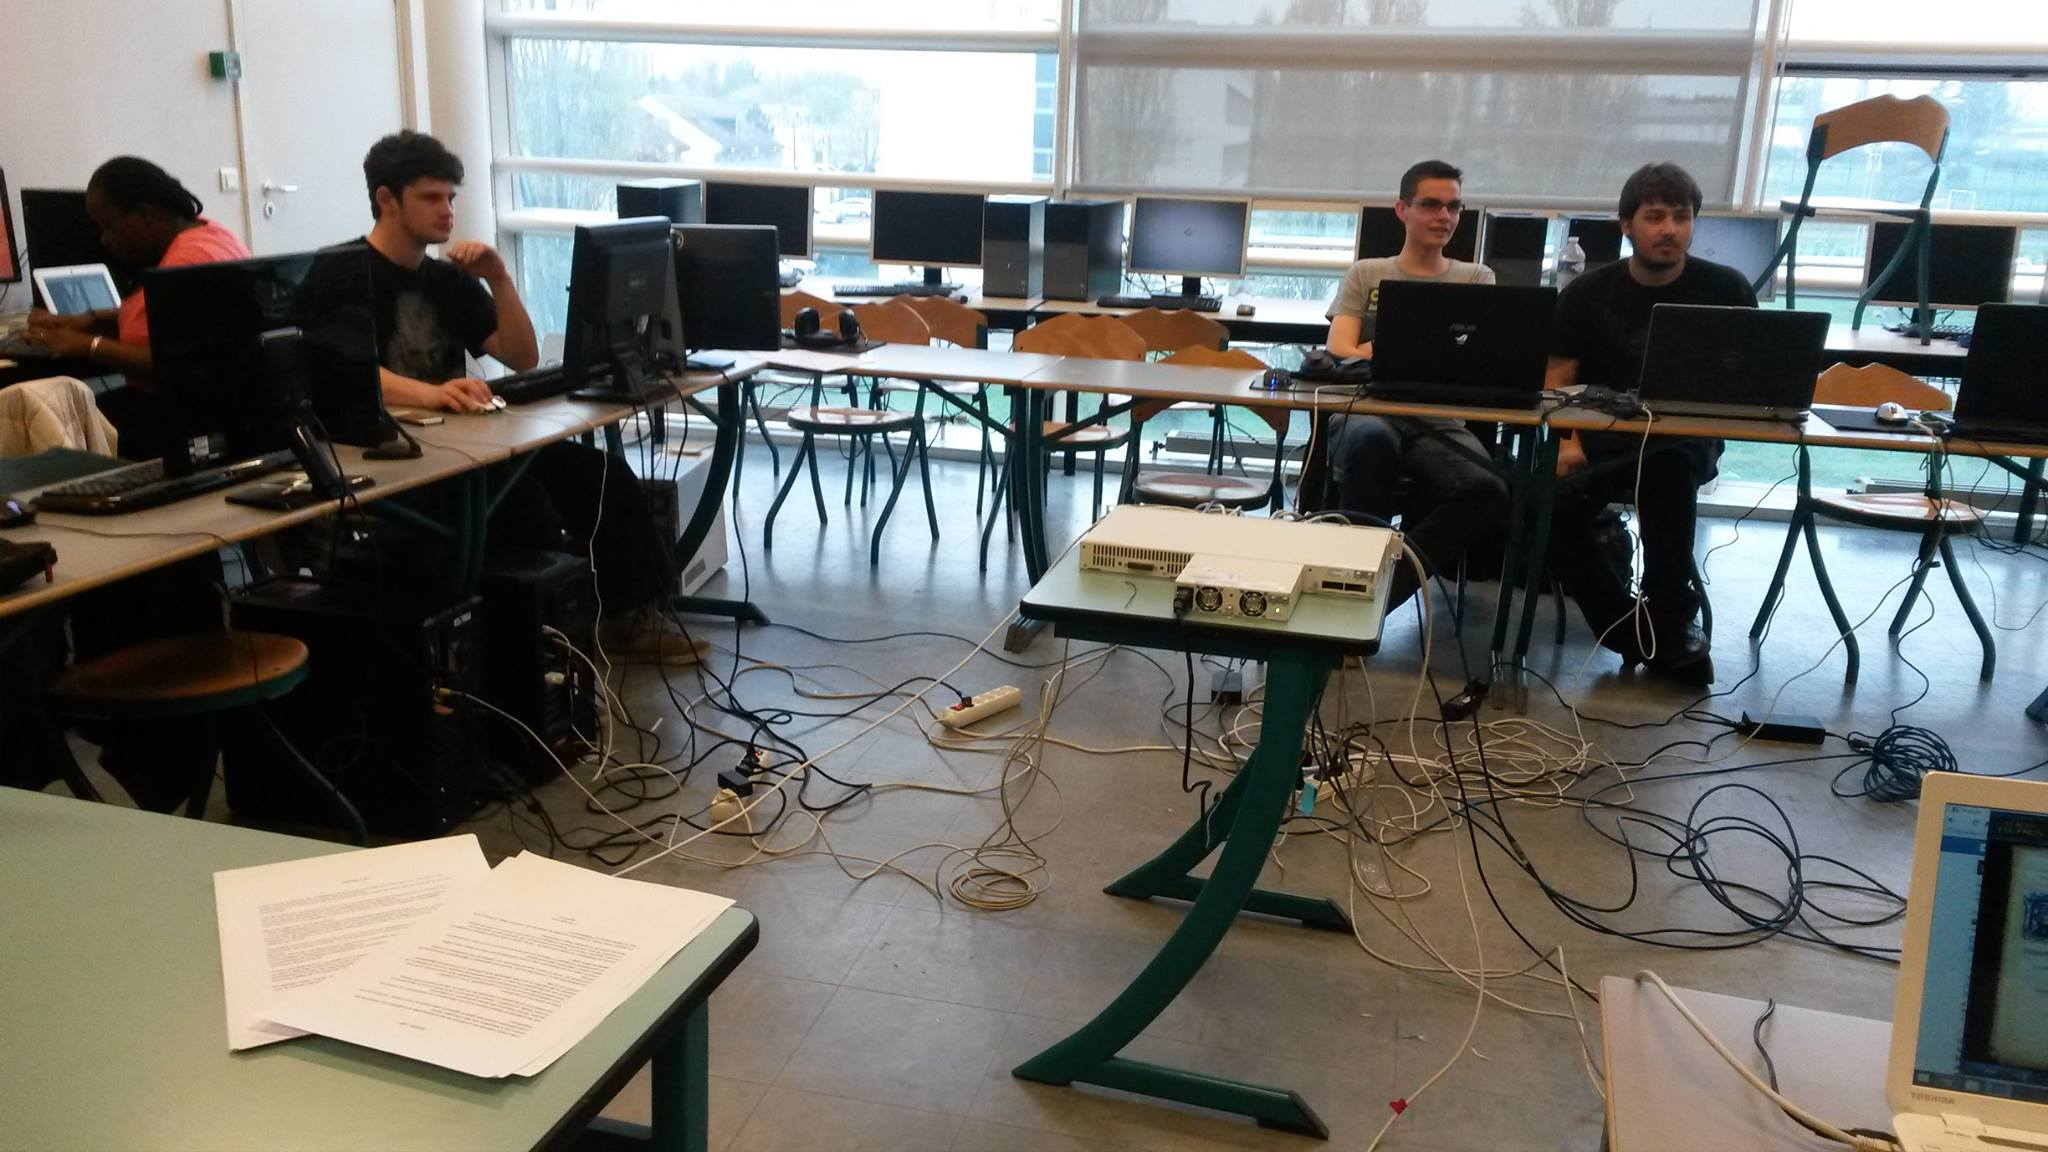
\includegraphics[width=0.8\textwidth]{images/versity1.jpg}
                \caption{VersityLAN \#1}
            \end{figure}
            
            En 2015-2016, l'association a continuer à développer ses LANs en y ajoutant de nouveaux tournois et en accueillant toujours plus de participants. En effet, la 3\up{ème} édition a réuni plus de 90 étudiants tandis que la 4\up{ème} édition a permis d'atteindre près de 130 participants.
            Ces nouvelles éditions ont permis à >ECHO de mettre en place un partenariat avec une autre association étudiante de l'Université de Cergy-Pontoise dédié aux jeux vidéo : LifeUp. LifeUp propose depuis maintenant trois éditions des tournois sur des jeux comme Smash Bros et l'univers Nintendo.
            
            \begin{figure}[ht]
                \centering
                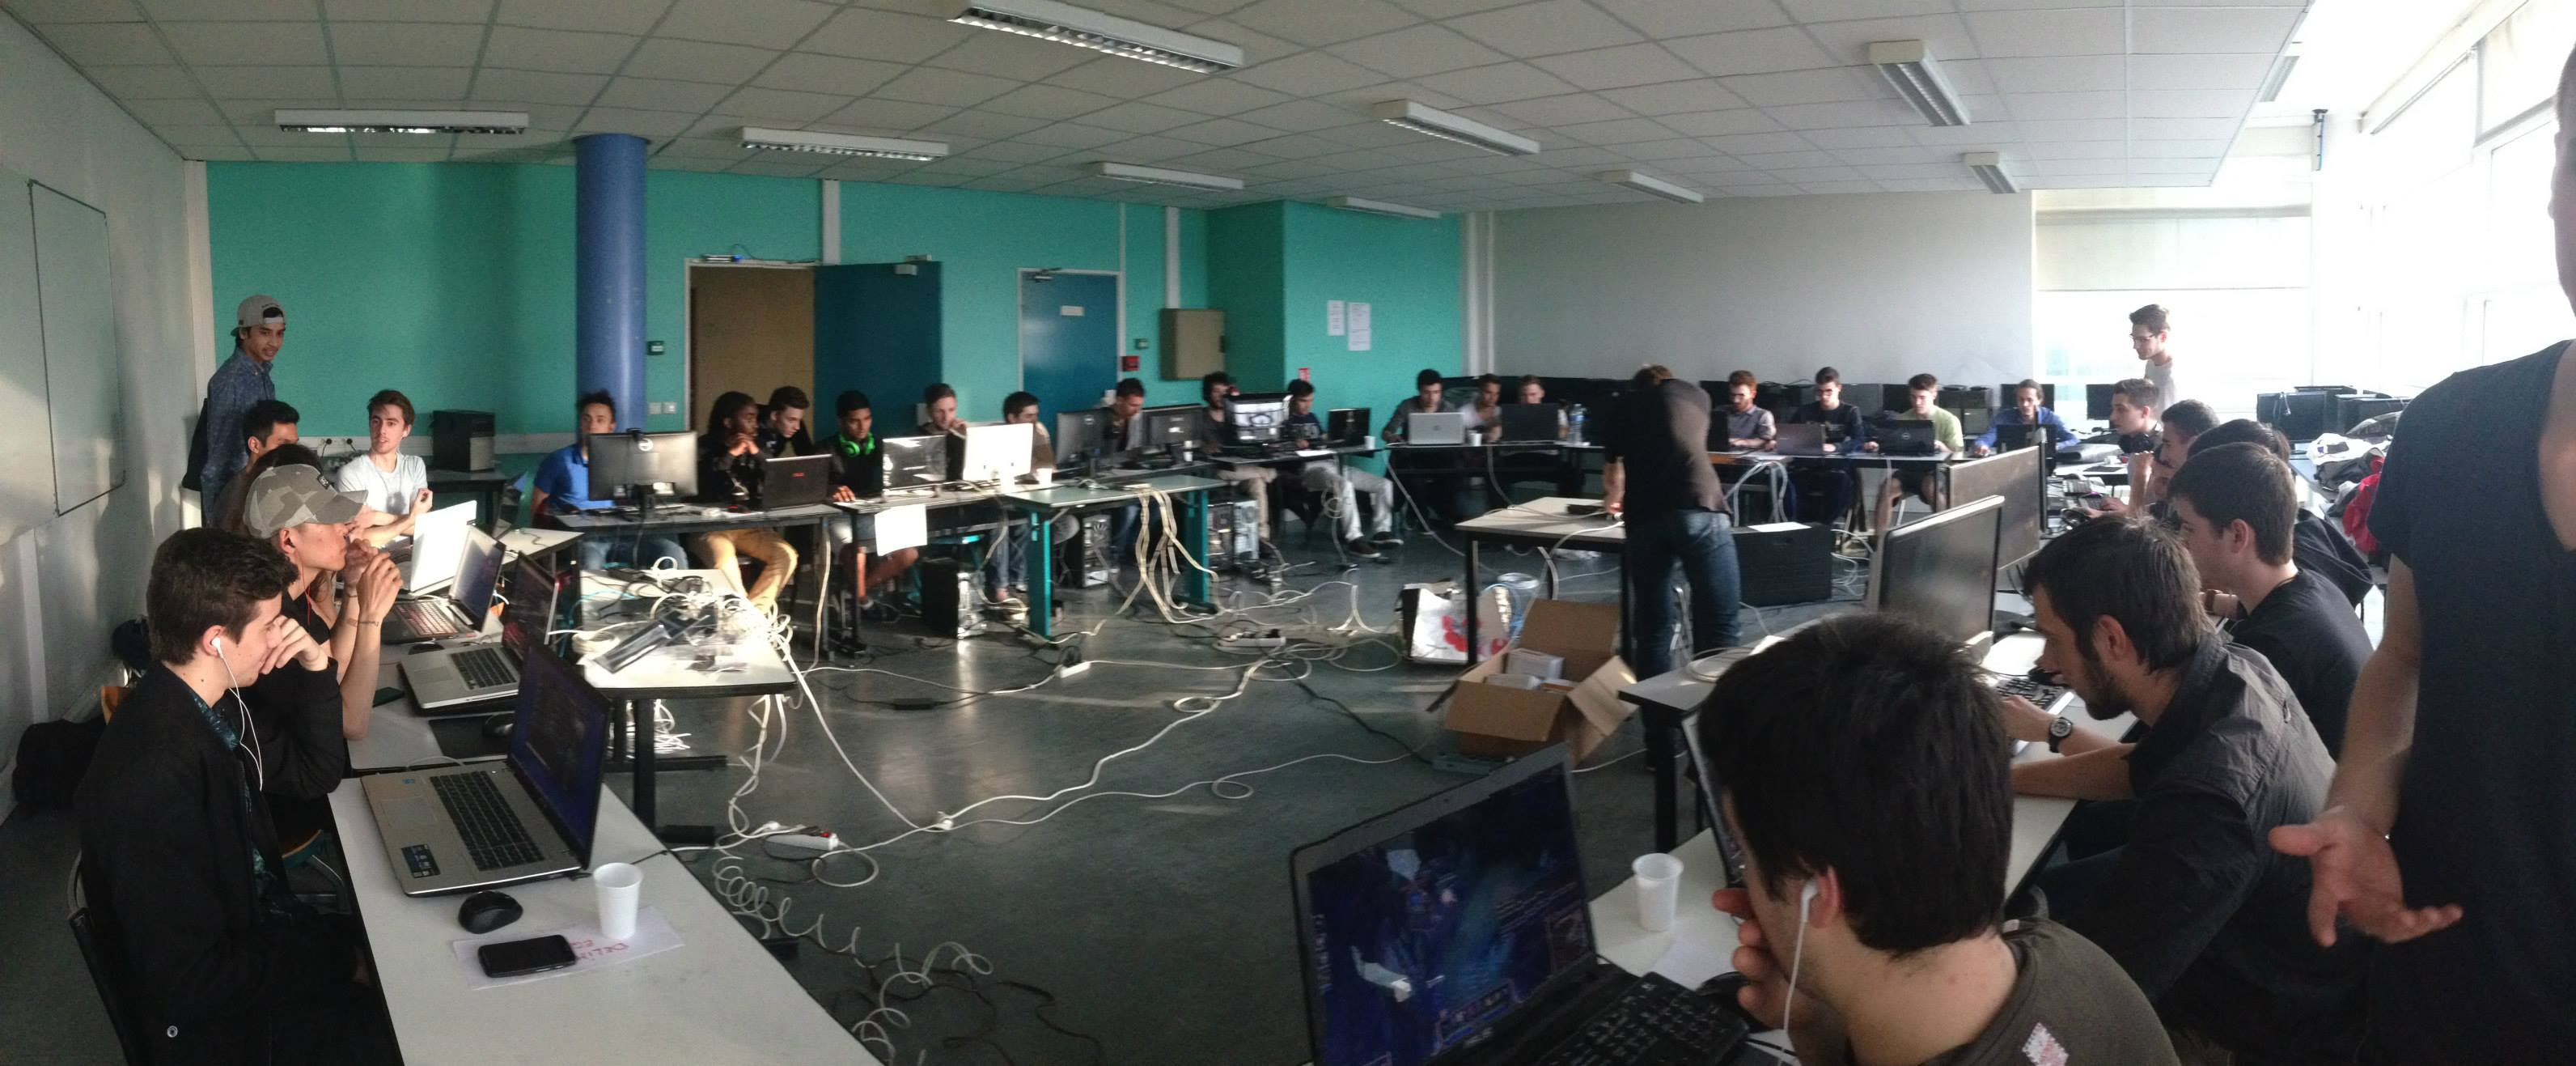
\includegraphics[width=1\textwidth]{images/versity3.jpg}
                \caption{VersityLAN \#3 tournoi LoL}
            \end{figure}
            
            \newpage
            
            La 3\up{ème} édition a permis de mettre en place un nouveau type de tournoi : le FFA, dont le principe est de laisser les joueurs non inscrits à des tournois de l'évènement s'organiser ensemble avec l'aide des organisateurs pour mettre en place un mini-tournoi sur le jeu de leurs choix. Par exemple lors de la 4\up{ème} édition, les joueurs inscrits en FFA ont organisé un tournoi sur Team Fortress 2.
            
            \begin{figure}[ht]
                \centering
                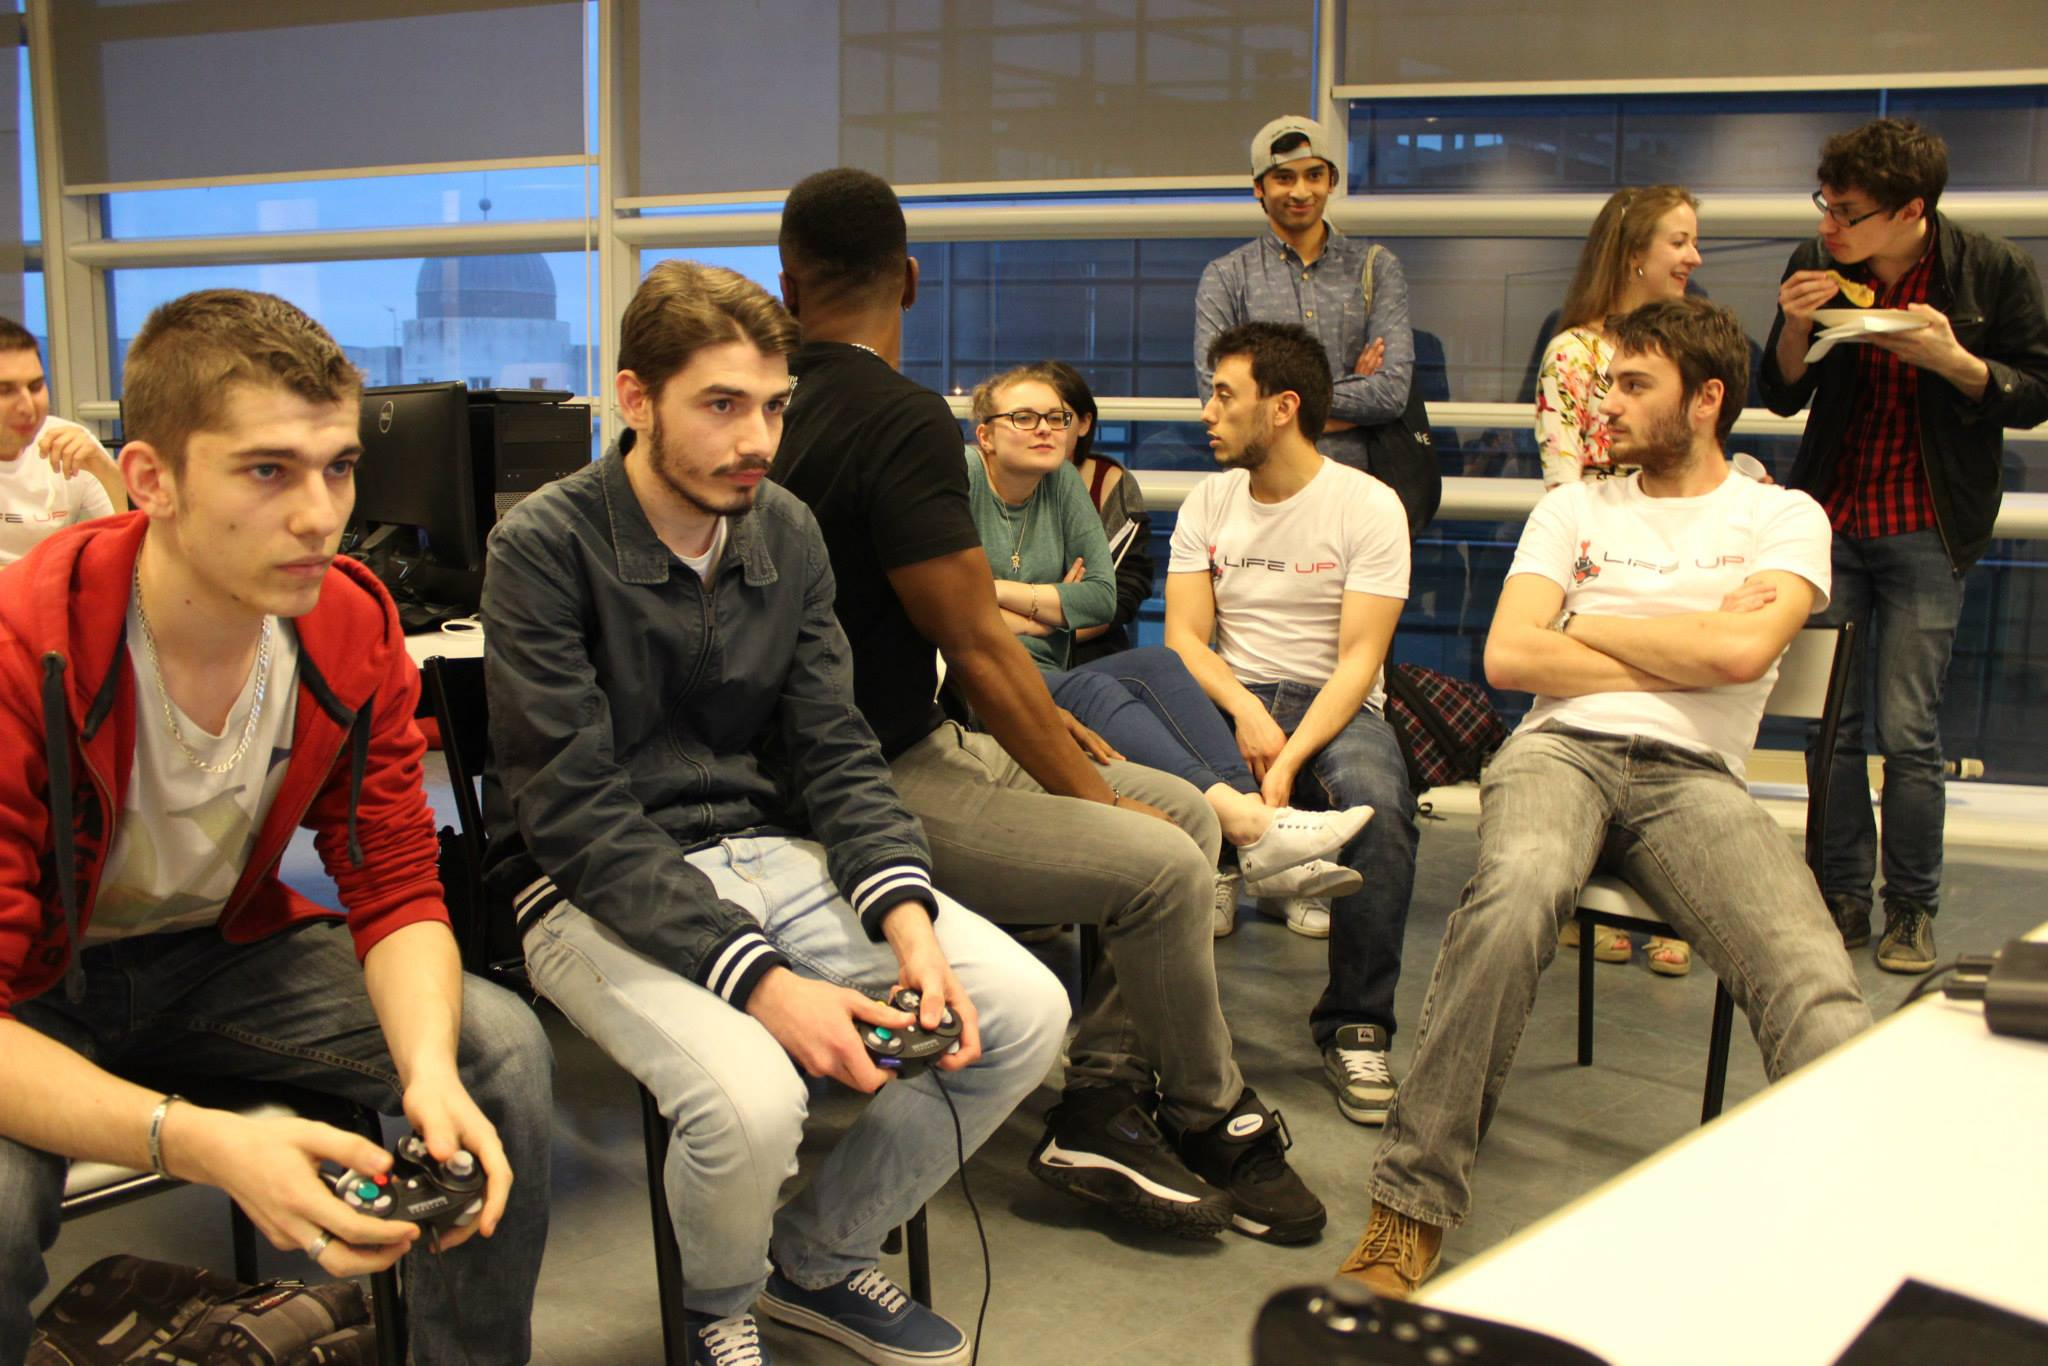
\includegraphics[width=0.65\textwidth]{images/versity3smash.jpg}
                \caption{VersityLAN \#3 tournoi Smash Bros}
            \end{figure}
            
            La dernière édition en date était la VersityLAN \#5 en février 2017 et a accueilli plus de 150 personnes. La grande nouveauté a été le rallongement de la durée de l'événement qui ne s'est pas déroulait de 18h à 00h, mais de 18h à 06h du matin permettant ainsi d'organiser des tournois plus conséquents.
            
            \begin{figure}[ht]
                \centering
                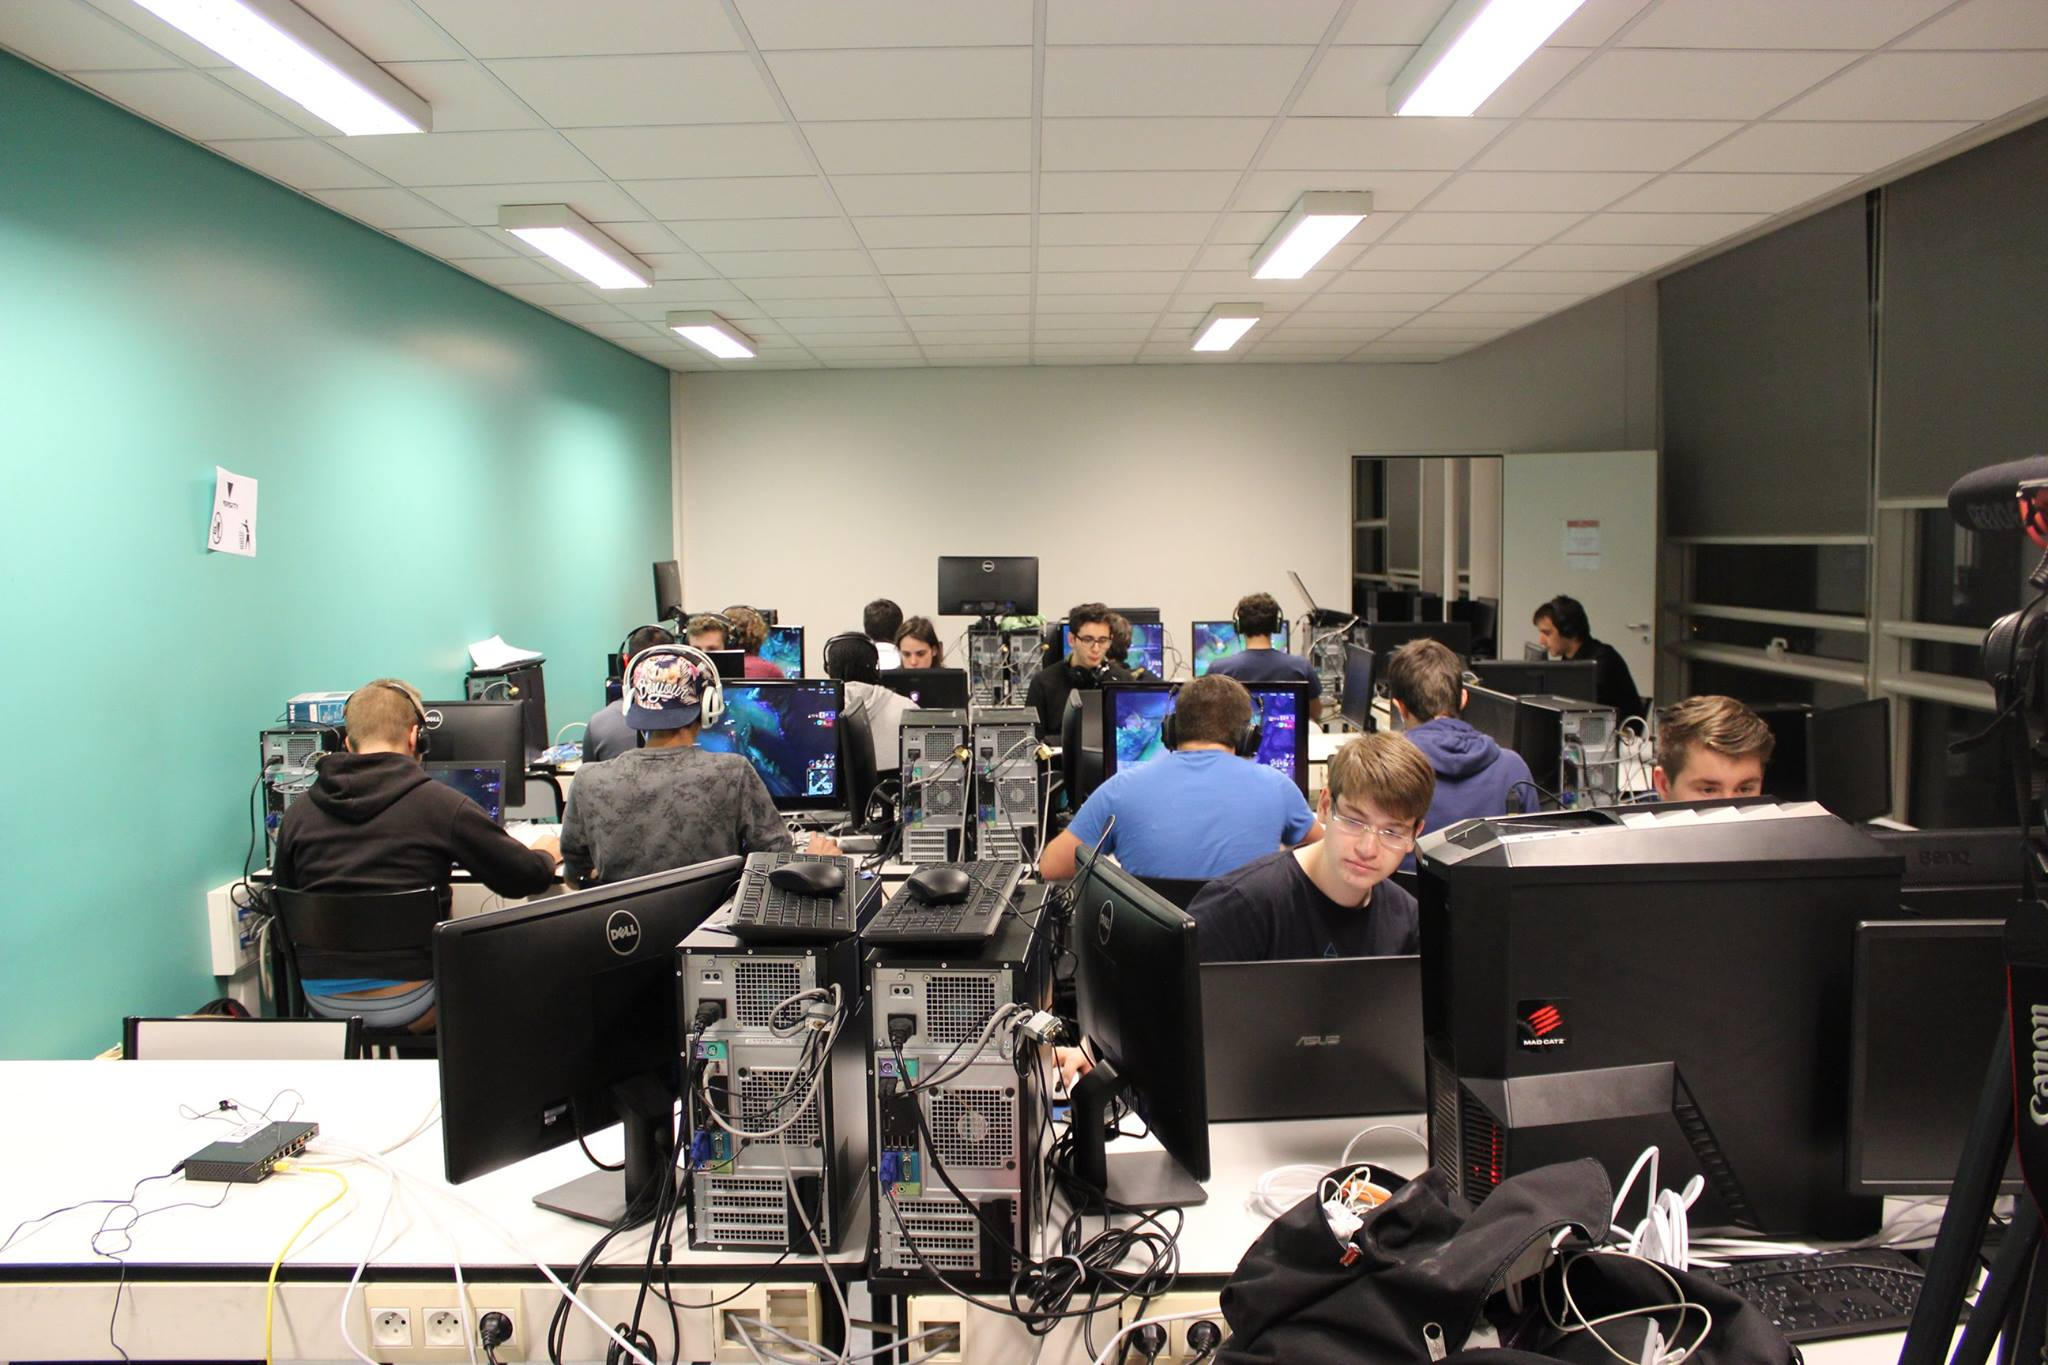
\includegraphics[width=0.62\textwidth]{images/versity5.jpg}
                \caption{VersityLAN \#5}
            \end{figure}
            
            
        
        
    
    \subsection{Musique électronique}
    
        Depuis l'année universitaire 2016-2017, >ECHO s'est diversifiée avec l'ajout d'un nouveau pôle dédié à la musique électronique. Les dirigeants de ces années, étant passionnés par la musique électronique et s'apercevant qu'au sein de l'Université de Cergy-Pontoise peu d'événements liés à cette culture étaient proposé malgré le nombre d'étudiants attirés, ont décidé de créer des événements autour de la musique électronique.
        
        Les manifestations proposées sont diverses mais le maître mot est le partage avec, par exemple, les réseaux sociaux où les membres de l'association partagent différentes musiques électroniques qu'ils ont découvertes ou encore en mettant en avant le contenu musical (production, DJ Set, etc.) des étudiants de l'Université de Cergy-Pontoise.
        
        \begin{figure}[ht]
            \centering
            
\includegraphics[width=0.65\textwidth]{images/logo_cadence.jpg}
            \caption{Logo Cadence}
        \end{figure}
            
        En mars 2017, l'association >ECHO a réalisé sa première "Cadence", un événement culturel et festif sur le format d'une soirée au sein même de l'Université de Cergy-Pontoise durant laquelle une scène a été monté dans le restaurant universitaire du site de Saint Martin et des artistes se sont produits durant des DJ Sets.
        
        \begin{figure}[ht]
            \centering
            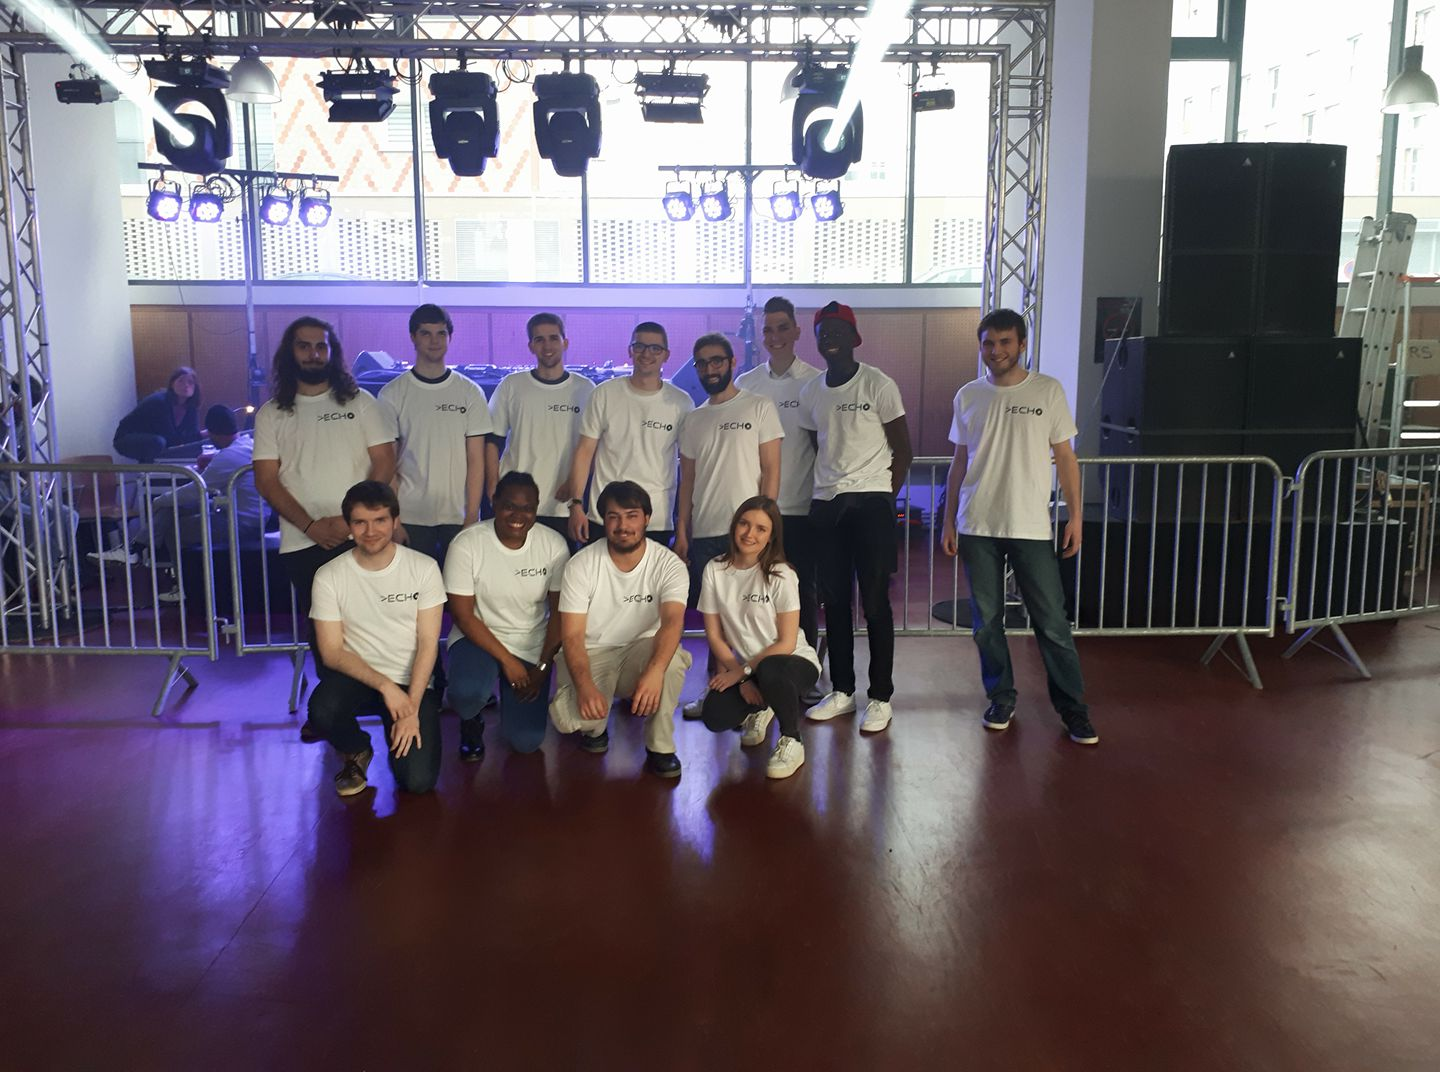
\includegraphics[width=0.62\textwidth]{images/cadencestaff.jpg}
            \caption{Cadence \#1}
        \end{figure}
        
        Plus de 150 étudiants étaient présents pour cette première édition, et c'était le premier événement de cette nature qu'a organisé >ECHO et l'Université de Cergy-Pontoise.


%%% Local Variables: 
%%% mode: latex
%%% TeX-master: "isae-report-template"
%%% End: 
\chapter{Le projet}
\label{sec:monstage}

\section{Concept}
    
\section{Inscription dans notre projet}

\section{Inscription dans le projet de la vie culturelle/étudiante universitaire}

\section{Nom de l'événement précis (ex: VersityLAN \#12, Cadence \#3)}
    
    \subsection{Informations pratiques}
    
    \subsection{Lieu et plan}
    
    \subsection{Association(s) partenaire(s)}
    
    \subsection{Prestataires}
    
    \subsection{Budget}
    
    \subsection{Risque et enjeux}
    
    
       
    
        



%%% Local Variables: 
%%% mode: latex
%%% TeX-master: "isae-report-template"
%%% End: 
\chapter*{Conclusion et perspectives}
\addcontentsline{toc}{chapter}{Conclusion}
\markboth{Conclusion}{Conclusion}
\label{sec:conclusion}


    
%%% Local Variables: 
%%% mode: latex
%%% TeX-master: "isae-report-template"
%%% End: 



\appendix

%\clearpage

\end{document}